\newpage
\section{Aufbau}
	\begin{figure}
        \centering
        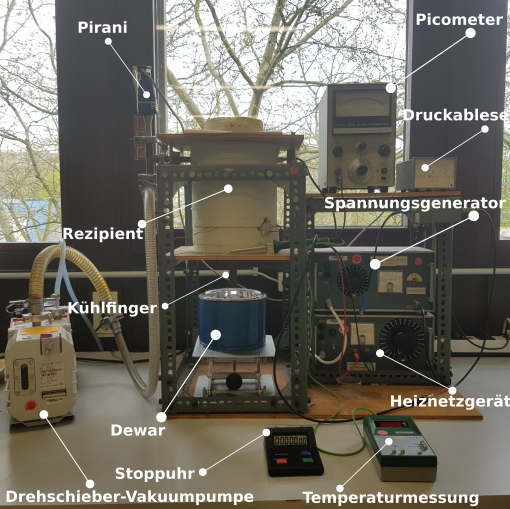
\includegraphics[width = 0.7\textwidth]{latex/images/Aufbau2.png}
        \caption{Bild eines analogen Versuchsaufbaus \cite{V48}.}
        \label{fig:Aufb2}
    \end{figure}
    \noindent
    In Abbildung \ref{fig:Aufb2}, ist ein Bild eines Versuchsaufbaus der analog zu dem verwendeten Aufbau ist, dargestellt. 
    In dem Aufbau auf dem Tisch ist unten rechts ein Heizgerät welches permanent an der Probe angeschlossen ist.
    Auf diesem steht ein Spannungsgenerator, der bei Bedarf an den Kondensator angeschlossen wird.
    Auf den beiden Generatoren steht rechts eine Anzeige zum Ablesen des Druckes im Rezipienten und links ein Amperemeter.\\
    In der Mitte des Aufbaus steht der Rezipient. 
	Dieser kann durch einen Kühlfinger auf der Unterseite mit dem darunter befindlichen Dewargefäß verbunden werden.
    Oberhalb des Rezipienten ist das Pirani Vakuummeter zu sehen.
	\begin{figure}
		\centering
		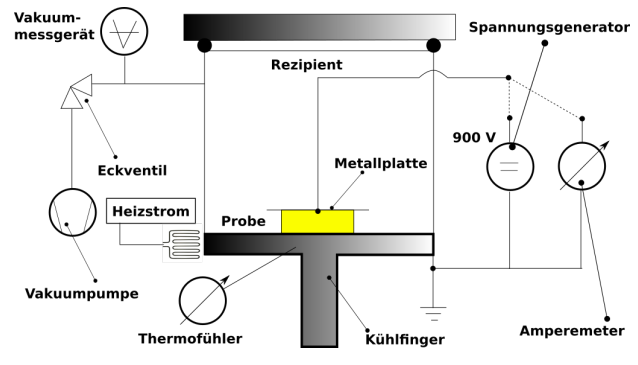
\includegraphics[width = 0.6\textwidth]{latex/images/Aufbau3.png}
		\caption{Skizze der Bauteile mit Querschnitt des Rezipienten \cite{V48}.}
		\label{fig:Aufb3}
	\end{figure}
	In Abbildung \ref{fig:Aufb3}, ist die Schaltzseichnung zu dem beschreibenen Aufbau mit einem Querschnitt des Vakuumkörpers dargestellt. 
	Hier ist zu sehen, wie der Kühlfinger direkt an der Probe anliegt und wie die Probe innerhalb des Kondensators positioniert ist.
     
\section{Durchführung}

    Um die charakteristischen Größen der Dipolrelaxation zu bestimmen, 
    werden zunächst die Dipole ausgerichtet, indem die Probe auf $\SI{50}{\celsius}$ aufgewärmt und dabei ein ein E-Feld mit einer Spannung $\SI{900}{\volt}$ angelegt wird.
    Sobald $\SI{50}{\celsius}$ in der Probe erreicht wurden kann die Probe nun bei weiterhin angeschaltetem E-Feld abgekühlt werden.
    Dazu wird das Dewargefäß mit flüssigem Stickstoff gefüllt und auf den Ständer gestellt.
    Der Ständer wird dann bis knapp unter die Probe hoch gedreht damit der Kühlfinger vom flüssigen Stickstoff eingeschlossen ist und die Probe abkühlt.\\
    Sobald die Probe auf $\SI{-50}{\celsius}$ abgekühlt wurde, kann nun das E-Feld abgeschalten werden, indem der Spannungsgenerator runter geregelt und abgeschalten wird.
    Nachdem die Spannung komplett abgefallen ist wird der Kondensator noch einmal für 10 Minuten an die Erdung des Ampermeters angeschlossen, damit auch wirklich alle Ladungen abgeflossen sind.\\
    Nun wird der Kondensator am Ampermeter angeschlossen, um den Depolarisationsstrom zu messen, und das Heizgerät eingeschalten.
    Für die erste Messreihe wird die Heizrate so eingestellt, dass sich die Temperatur der Probe um $\SI{1.5}{\celsius}$ pro Minute erhöht.
    Es wird im $\SI{60}{\second}$ Takt die Temperatur und der Strom dokumentiert, bis die Temperatur der Probe wieder $\SI{50}{\celsius}$ erreicht. 
    Die zweite Messreihe wird nun vorbereitet, in dem bei einer Probentemperatur von mindestens $\SI{50}{\celsius}$, das E-Feld bei einer Spannung von $\SI{900}{\volt}$ für mindestens 15 Minuten eingeschaltet bleibt.
    Die restliche Versuchsdurchführung ist nun exakt wie bei der ersten Messreihe, nur mit einer Heizrate von $\SI{2}{\celsius}$ pro Minute.
